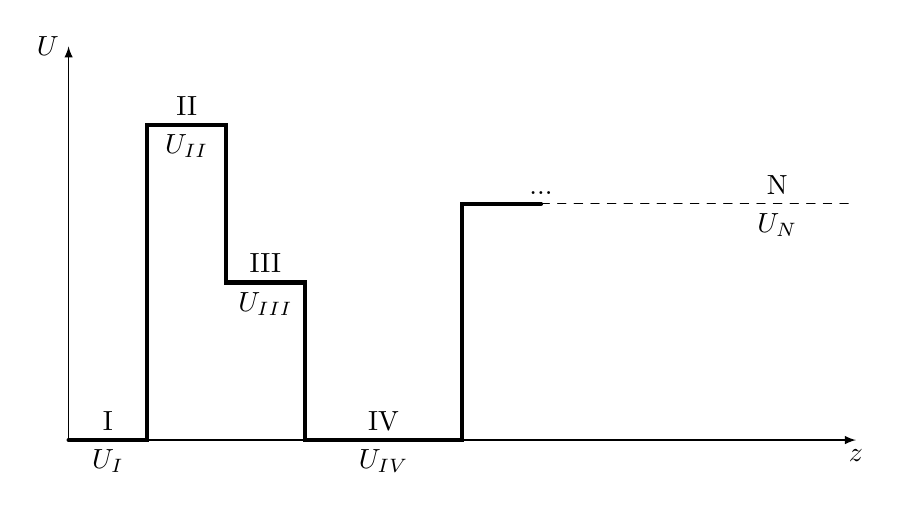
\begin{tikzpicture}[scale=1,cap=round,>=latex]
	\draw [<->] (-5, 5) -- (-5, 0) -- (5, 0);
	\node [left] at (-5, 5) {$U$};
	\node [below] at (5, 0) {$z$};
	
	\draw [line width=1.5] (-5, 0) -- (-4, 0) -- 
							(-4, 4) -- (-3, 4) -- 
							(-3, 2) -- (-2, 2) --
							(-2, 0) -- (0, 0) --
							(0, 3) -- (1, 3);
	\draw [dashed] (1, 3) -- (5, 3);
	
	\node [above] at (-4.5, 0) {I};
	\node [below] at (-4.5, 0) {$U_I$};

	\node [above] at (-3.5, 4) {II};
	\node [below] at (-3.5, 4) {$U_{II}$};
	
	\node [above] at (-2.5, 2) {III};
	\node [below] at (-2.5, 2) {$U_{III}$};

	\node [above] at (-1, 0) {IV};
	\node [below] at (-1, 0) {$U_{IV}$};
	
	\node [above] at (1, 3) {...};
		
	\node [above] at (4, 3) {N};
	\node [below] at (4, 3) {$U_{N}$};


	%\node [below] at (-1, 0) {$-\frac{d}{2}$};
	%\node [below] at (0, 0) {$\frac{d}{2}$};
	
\end{tikzpicture}